% Research paper: Hindi-English code-mixed meeting assistant.
%
% Build:   powershell -File build.ps1   (or latexmk -pdf main.tex, or Overleaf)
% Results: tables/ and figures/ are generated by the evaluation code and are
%          pulled in automatically when present; never edit them by hand.
%
% Placeholders are written with \pending{...}. They print in red while
% drafting; a submission build (build.ps1 -Final) stops at the first one left,
% so a draft can never be submitted by accident.
\documentclass[conference]{IEEEtran}

\usepackage[T1]{fontenc}
\usepackage[utf8]{inputenc}
\usepackage{cite}
\usepackage{amsmath,amssymb}
\usepackage{graphicx}
\usepackage{booktabs}
\usepackage{multirow}
\usepackage{xcolor}
\usepackage{url}
\usepackage{tikz}
\usetikzlibrary{arrows.meta,positioning,fit,calc}
\usepackage[hidelinks]{hyperref}

% ---------------------------------------------------------------------------
% Drafting aids
% ---------------------------------------------------------------------------
\newif\iffinal
% Submission build (`build.ps1 -Final` defines \SUBMISSION): any \pending,
% or any result table or figure not yet generated, stops the build.
\ifdefined\SUBMISSION\finaltrue\fi

\newcommand{\pending}[1]{%
  \iffinal\errmessage{Unfinished placeholder: #1}\else\textcolor{red}{[#1]}\fi}

% A results table or figure produced by `meeting-assistant paper build`.
% Until the file exists, a visible box says what will go there.
\newcommand{\pendingbox}[1]{%
  \iffinal\errmessage{Missing generated result: #1}\else
  \fbox{\parbox{0.92\columnwidth}{\centering\small\textcolor{red}{%
    Pending: #1\\(generated by \texttt{meeting-assistant paper build})}}}\fi}
\newcommand{\resulttable}[2]{\IfFileExists{tables/#1.tex}{\input{tables/#1.tex}}{\pendingbox{#2}}}
\newcommand{\resultfigure}[3][\columnwidth]{%
  \IfFileExists{figures/#2.pdf}{\includegraphics[width=#1]{figures/#2.pdf}}{\pendingbox{#3}}}

% Names used throughout, so they stay consistent.
\newcommand{\system}{\textsc{HinglishMeet}}
\newcommand{\werraw}{$\mathrm{WER}_{\mathrm{raw}}$}
\newcommand{\werrom}{$\mathrm{WER}_{\mathrm{rom}}$}
\newcommand{\cerraw}{$\mathrm{CER}_{\mathrm{raw}}$}

\begin{document}

\title{\system: A Reproducible, Fully Local Pipeline for Understanding
Hindi--English Code-Mixed Meetings}

\author{%
\IEEEauthorblockN{\pending{Author 1}, \pending{Author 2}, \pending{Author 3}}
\IEEEauthorblockA{\pending{Department}, \pending{Institution}\\
\pending{City, Country}\\
\pending{email addresses}}
}

\maketitle

\begin{abstract}
Meetings in Indian workplaces and classrooms are routinely conducted in
Hindi--English code-mixed speech (``Hinglish''), yet meeting assistants are
built and evaluated almost exclusively on monolingual English, and most depend
on cloud services that cannot be used for confidential recordings. We present
\system{}, an open-source meeting assistant that runs entirely on a single
machine and turns a code-mixed recording into a speaker-attributed,
language-tagged transcript, a Romanized Hinglish rendering, a summary and a list
of action items, both for uploaded recordings and live from a microphone. The
pipeline integrates Whisper large-v3 for recognition, pyannote for speaker
diarization, a script-based language tagger and a locally served
7B-parameter language model, and is designed around two constraints that
code-mixing makes pressing: language identification must precede any
transliteration, and the transliteration model must never be used to score
itself. Every run records the code version, a hash of all output-affecting
settings, versioned prompts and the input's checksum, and runs that mix
configurations are excluded from evaluation automatically, so every number
reported here can be traced to the runs that produced it and regenerated with
one command. On a dataset of \pending{N} code-mixed meetings (\pending{H} hours,
\pending{2--4} speakers) we report word and character error rates under
script-aware and script-normalized scoring (\pending{X}\,\% and
\pending{Y}\,\% WER), diarization error rate (\pending{Z}\,\%), language
identification accuracy (\pending{A}\,\%, $\kappa=$\,\pending{K} between
annotators), summary ROUGE and action-item $F_1$, together with ablations over
model size, quantization and pipeline design, and real-time factors on
commodity CPU and GPU hardware.
\end{abstract}

\begin{IEEEkeywords}
code-switching, Hindi--English, meeting transcription, speaker diarization,
summarization, large language models, reproducibility
\end{IEEEkeywords}

\section{Introduction}
\label{sec:introduction}

Code-switching, the alternation between two languages within a conversation or a
single sentence, is the norm rather than the exception in multilingual
communities~\cite{sitaram2019survey}. In Indian professional and academic
settings, meetings mix Hindi and English freely: a sentence such as
``\textit{release Friday ko hoga, testing kal tak}'' (``the release will be on
Friday, testing by tomorrow'') carries its decision in English nouns and its
commitment in Hindi grammar. Automatic meeting assistants, which transcribe a
meeting, attribute speech to speakers and distil it into a summary and action
items, are now common for English, but three properties of Hindi--English
meetings make them a poor fit for existing tools.

First, \emph{the script is ambiguous}. Hindi words may be written in Devanagari
or in Latin script, and a speech recognizer may emit either, even within one
utterance. A transcript that is correct word for word can still score close to
100\,\% word error rate if its reference uses the other script. Second,
\emph{downstream steps interact}. Transliterating Hindi into Latin script, which
makes a transcript readable to colleagues who do not read Devanagari, destroys
the evidence a script-based language identifier relies on; done in the wrong
order, every segment silently becomes ``English''. Third, \emph{recordings are
often confidential}, so an assistant that uploads audio to a cloud service is
frequently not an option.

This paper presents \system{}, a meeting assistant for Hindi--English
code-mixed speech that runs entirely on one machine with open-weight models, and
a reproducible evaluation of it. Our contributions are:

\begin{enumerate}
  \item \textbf{An integrated, fully local pipeline}
    (Section~\ref{sec:system}) combining Whisper large-v3~\cite{radford2023whisper},
    pyannote speaker diarization~\cite{bredin2020pyannote,plaquet2023powerset},
    script-based language identification and a locally served
    7B-parameter language model~\cite{qwen2024qwen25} to produce speaker-attributed,
    language-tagged transcripts, Romanized Hinglish, summaries and action items,
    for both recorded and live meetings.
  \item \textbf{Design rules for code-mixed pipelines}, enforced in code rather
    than by convention: language identification precedes transliteration;
    transliteration is restricted to script conversion and may not correct
    recognition errors; and the evaluation uses a deterministic transliterator,
    never the system's own, so the system is not used to score itself.
  \item \textbf{A provenance design that makes results auditable}
    (Section~\ref{sec:provenance}): each run records the code commit, a hash of
    every output-affecting setting, prompt versions and the input's checksum;
    runs whose stages were produced under different configurations are excluded
    from evaluation automatically; and all tables and figures in this paper are
    generated from stored runs by a single command.
  \item \textbf{An evaluation study} (Sections~\ref{sec:evaluation}
    and~\ref{sec:results}) covering seven families of metrics (recognition,
    diarization, cross-chunk speaker identity, language identification,
    summarization, action-item extraction and system efficiency) on
    \pending{N} annotated code-mixed meetings, with annotator agreement,
    bootstrap confidence intervals and ablations over the choices that most
    affect quality and cost.
\end{enumerate}

The code, the annotation protocol and the generated results are released at
\pending{repository URL}.

\section{Related Work}
\label{sec:related}

\paragraph{Code-switched speech recognition}
Sitaram et al.~\cite{sitaram2019survey} survey code-switched speech and language
processing and identify the scarcity of transcribed code-mixed speech and the
inconsistency of its written form as the central obstacles. The MUCS~2021
challenge~\cite{diwan2021mucs} established benchmarks for Hindi--English and
Bengali--English code-switched recognition and noted the need to normalize
script before scoring. Large weakly supervised models such as
Whisper~\cite{radford2023whisper} recognize Hindi and English without
task-specific training, but their output script for Hindi is not controlled,
which our evaluation protocol addresses explicitly.

\paragraph{Long-form transcription and diarization}
pyannote.audio~\cite{bredin2020pyannote} provides neural building blocks for
speaker diarization; its current pipeline combines powerset segmentation
\cite{plaquet2023powerset} with speaker embeddings~\cite{wang2023wespeaker} and
clustering~\cite{bredin2023pyannote21}. WhisperX~\cite{bain2023whisperx} couples
Whisper with diarization for time-accurate long-form transcripts. Diarization is
scored with the diarization error rate (DER) introduced in the NIST Rich
Transcription evaluations~\cite{fiscus2006rt}, computed here with
pyannote.metrics~\cite{bredin2017pyannotemetrics}. These systems target
monolingual or language-agnostic audio; we study their behaviour on code-mixed
meetings and add speaker identity resolution across the chunks of a live
session.

\paragraph{Meeting summarization}
Meeting corpora such as AMI~\cite{carletta2005ami} and ICSI~\cite{janin2003icsi}
and benchmarks such as QMSum~\cite{zhong2021qmsum} have driven meeting
summarization research, overwhelmingly in English. Summaries are commonly scored
with ROUGE~\cite{lin2004rouge}. Open-weight instruction-tuned models such as
Qwen2.5~\cite{qwen2024qwen25} and Llama~3~\cite{grattafiori2024llama3} now make
it practical to summarize and extract action items locally; we evaluate two such
models on code-mixed transcripts.

\paragraph{Reproducibility}
Pineau et al.~\cite{pineau2021reproducibility} document how often published
machine-learning results cannot be reproduced and argue for recording code
versions, configurations and data provenance. Our system applies these practices
at the level of individual pipeline runs, so that each reported number can be
traced to the runs, code and settings that produced it.

\pending{Add closest prior work on Hinglish meeting assistants or code-mixed
summarization, if any is found in the literature search.}

\section{System}
\label{sec:system}

\begin{figure*}[t]
\centering
% Scaled to the text width, so the diagram can never run into the margin.
\resizebox{\textwidth}{!}{%
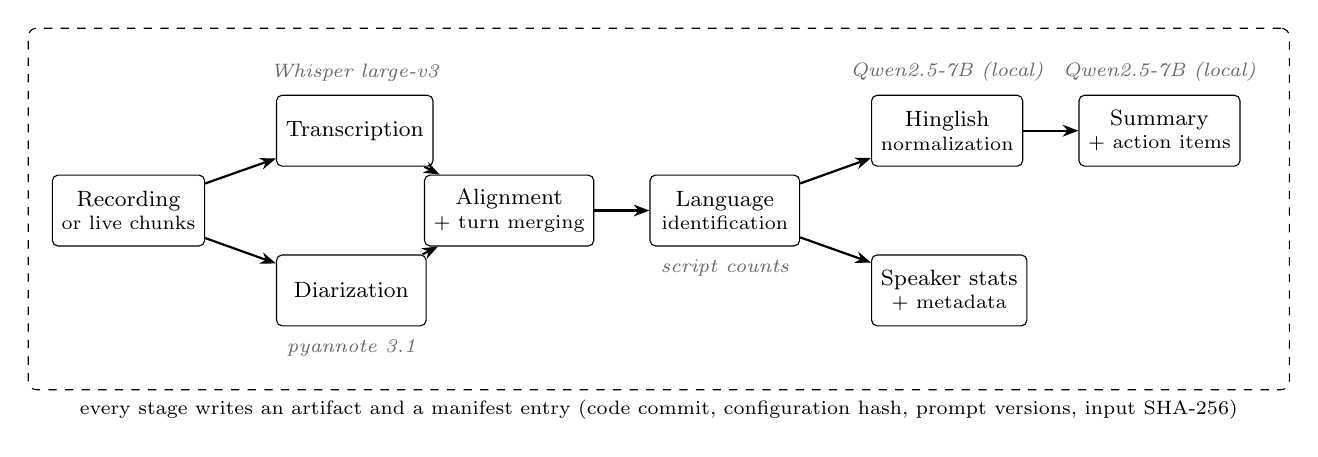
\begin{tikzpicture}[
  node distance=5mm and 7mm,
  stage/.style={draw, rounded corners=2pt, align=center, font=\footnotesize,
                minimum height=9mm, minimum width=19mm, fill=white},
  model/.style={font=\scriptsize\itshape, text=black!60},
  arrow/.style={-{Stealth[length=2mm]}, thick},
]
  \node[stage] (audio) {Recording\\[-1pt]\scriptsize or live chunks};
  \node[stage, above right=1mm and 9mm of audio] (asr) {Transcription};
  \node[stage, below right=1mm and 9mm of audio] (dia) {Diarization};
  \node[stage, right=9mm of $(asr)!0.5!(dia)$] (align) {Alignment\\[-1pt]\scriptsize + turn merging};
  \node[stage, right=of align] (lid) {Language\\[-1pt]\scriptsize identification};
  \node[stage, above right=1mm and 9mm of lid] (norm) {Hinglish\\[-1pt]\scriptsize normalization};
  \node[stage, below right=1mm and 9mm of lid] (stats) {Speaker stats\\[-1pt]\scriptsize + metadata};
  \node[stage, right=of norm] (sum) {Summary\\[-1pt]\scriptsize + action items};

  \node[model, above=0.5mm of asr] (m1) {Whisper large-v3};
  \node[model, below=0.5mm of dia] (m2) {pyannote 3.1};
  \node[model, above=0.5mm of norm] (m3) {Qwen2.5-7B (local)};
  \node[model, above=0.5mm of sum] (m4) {Qwen2.5-7B (local)};
  \node[model, below=0.5mm of lid] {script counts};

  \draw[arrow] (audio) -- (asr);
  \draw[arrow] (audio) -- (dia);
  \draw[arrow] (asr) -- (align);
  \draw[arrow] (dia) -- (align);
  \draw[arrow] (align) -- (lid);
  \draw[arrow] (lid) -- (norm);
  \draw[arrow] (lid) -- (stats);
  \draw[arrow] (norm) -- (sum);

  \node[draw, dashed, rounded corners=3pt, inner sep=3mm, fit=(audio)(asr)(dia)(sum)(stats)(m1)(m2)(m3)(m4),
        label={[font=\scriptsize]below:{every stage writes an artifact and a manifest entry
        (code commit, configuration hash, prompt versions, input SHA-256)}}] {};
\end{tikzpicture}%
}
\caption{Pipeline of \system{}. Transcription and diarization both read the
audio; alignment assigns speakers to recognized text; language identification
runs on the original script \emph{before} Hinglish normalization; summaries and
action items are produced from the normalized transcript. All models run on the
local machine.}
\label{fig:pipeline}
\end{figure*}

\system{} is a Python package exposing a command-line interface, an HTTP API and
a web interface over one pipeline (Fig.~\ref{fig:pipeline}). Each stage is a
function from input artifacts to one output artifact, declared with the
artifacts it requires so that the orchestrator, not the caller, enforces the
order. Stages write JSON artifacts into a directory per run; a SQLite index over
those directories serves queries but can always be rebuilt from them.

\subsection{Speech recognition}
Recognition uses Whisper large-v3~\cite{radford2023whisper} through
faster-whisper~\cite{fasterwhisper}, a CTranslate2 reimplementation, with beam
search (width~5) and Whisper's voice-activity filter to suppress hallucinated
text in silence. The model runs with 8-bit weights on CPU (\texttt{int8}) or
8-bit weights with 16-bit activations on GPU (\texttt{int8\_float16}). Hindi
segments are emitted in Devanagari or Latin script at the model's discretion;
the pipeline keeps the recognizer's output unmodified as the raw transcript.

\subsection{Diarization, alignment and turns}
Speaker diarization uses the pyannote speaker-diarization~3.1
pipeline~\cite{bredin2023pyannote21,plaquet2023powerset}, optionally given the
number of speakers. Each recognized segment is assigned the speaker whose turns
overlap it the longest; a segment with no overlapping turn is labelled
\textsc{unknown} rather than guessed. Consecutive segments of the same speaker
are merged into turns, but never across an \textsc{unknown} segment.

\subsection{Speaker identity across chunks}
In live mode each chunk is diarized independently, so the label
``SPEAKER\_00'' in one chunk need not denote the same person in the next. A
speaker registry resolves chunk-local labels to session-wide identities: for
each local label it embeds the label's longest turn with a
WeSpeaker ResNet34 model~\cite{wang2023wespeaker} and assigns it to the
registered speaker with the highest cosine similarity, if that similarity is at
least $\theta=0.75$; otherwise a new speaker is registered. A matched speaker's
centroid is updated as $c \leftarrow (1-\alpha)c + \alpha e$ with $\alpha=0.3$.
Windows shorter than 1\,s give unstable embeddings and are left unresolved
rather than merged, keeping their chunk-local label visibly prefixed so that
uncertainty is not hidden. The threshold $\theta$ is studied in
Section~\ref{sec:results}.

\subsection{Language identification}
Each segment is tagged \textsc{Hindi}, \textsc{English} or \textsc{Code-Mixed}
from its script: let $r$ be the fraction of script-bearing words written in
Devanagari. A segment is \textsc{Hindi} if $r \geq 0.85$, \textsc{English} if
$r \leq 0.15$ and \textsc{Code-Mixed} otherwise. A segment with a single
script-bearing word takes that word's script, and one with none (numbers or
punctuation only) defaults to \textsc{English}, a default recorded as such. The rule is deliberately
simple and auditable, but it can only see what the script shows: Hindi that the
recognizer has already written in Latin script is tagged \textsc{English}. For
the same reason, this stage must run before transliteration. The pipeline
enforces the order, since normalization declares the tagged transcript as its
input and copies the tags instead of recomputing them.

\subsection{Hinglish normalization}
For readers who do not read Devanagari, a local language model rewrites each
segment in Romanized Hinglish. The prompt restricts the model to script
conversion: it must not translate, add, remove or correct words. Correcting
recognition errors at this step would make recognition quality look better than
it is and would contaminate the evaluation of both steps.

\subsection{Summaries and action items}
A local language model (Qwen2.5-7B-Instruct~\cite{qwen2024qwen25}, served by
Ollama~\cite{ollama}, temperature~0.1) produces a summary with highlights and
decisions, and a list of action items with an assignee, a task and a deadline
when one is stated, both from the speaker-attributed transcript and both as
JSON, with one retry on unparseable output. Prompts are versioned constants
recorded in each run, so a prompt change is visible in the provenance of every
result produced with it. Speaker statistics (speaking time, share, turns,
words, words per minute) and meeting metadata are computed deterministically.

\subsection{Live mode}
In live mode, audio from a microphone is segmented at pauses by
WebRTC voice-activity detection~\cite{webrtcvad} (aggressiveness~2): a chunk
ends at a pause of at least 1.2\,s and lasts between 1 and 45\,s, so chunk
boundaries rarely cut a word or a turn. Recording and processing are decoupled
through a queue: the capture thread only enqueues chunks, and a single worker
thread owns every model, so audio is never dropped while a chunk is being
processed. Stopping a session drains the queue before the final stages run. Each
live run records the number of chunks recorded and processed, the maximum
backlog and the real-time factor, which together show whether the system kept
up with speech.

\subsection{Provenance and reproducibility}
\label{sec:provenance}
Every run directory holds a manifest that records, at the start of the run: the
code commit and whether the working tree had uncommitted changes; the software
environment; a hash of every setting that can change an output (model names,
devices and numeric precision, thresholds, prompt versions); the input's file
name, size and SHA-256 checksum; and whether the input is real or synthetic
audio. Each stage appends its status, duration, outputs and counts.

Resuming an interrupted run re-records the environment. If the configuration
hash or input checksum changed, the resume is refused unless explicitly
overridden, and an overridden run is flagged as mixed. The evaluation scores only
runs on real audio whose stages were all produced under one configuration and
one code version; others are reported as ineligible with the reason. Because
recognizer output is affected by numeric precision, CPU (\texttt{int8}) and GPU
(\texttt{int8\_float16}) runs have different configuration hashes and are never
pooled. All tables and figures in Section~\ref{sec:results} are generated from
the stored runs by one command, \texttt{meeting-assistant paper build}.

\subsection{Deployment}
The system runs on a laptop CPU or, through a container with GPU access, on a
consumer GPU; the language model is served locally, so no audio or text leaves
the machine. A web interface supports uploading recordings, live sessions,
waveform playback synchronized with the transcript and search across meetings;
each user account sees only its own recordings and meetings.

\section{Evaluation Methodology}
\label{sec:evaluation}

\subsection{Dataset}
We recorded \pending{N} meetings of 1--3 minutes each with 2--4 participants,
\pending{total duration}, chosen to span four conditions: Hindi-dominant,
English-dominant and balanced code-mixed conversation, and one adverse condition
(\pending{background noise / distant microphone}). Table~\ref{tab:dataset}
lists each clip. Participants gave \pending{informed consent; ethics approval
details}. \pending{Recording setup: device, room, sample rate.}

\begin{table}[t]
\centering
\caption{Evaluation clips.}
\label{tab:dataset}
\resulttable{dataset}{per-clip duration, speakers, language mix, condition}
\end{table}

\subsection{Annotation}
For every clip, annotators produced: (i)~a verbatim reference transcript, in
the script each word was spoken in (Devanagari for Hindi, Latin for English);
(ii)~speaker turn boundaries, marked as labelled regions in Audacity and
converted to RTTM; (iii)~a language tag per segment (\textsc{Hindi},
\textsc{English}, \textsc{Code-Mixed}); (iv)~the action items as (assignee,
task, deadline) triples; and (v)~one reference summary. A second annotator
independently labelled the language tags of \pending{20}\,\% of the segments;
we report Cohen's $\kappa$~\cite{cohen1960kappa} for that subset.
\pending{Annotator background and guidelines.}

\subsection{Metrics}
\paragraph{Recognition}
Word error rate is
$\mathrm{WER} = (S + D + I)/N$ for $S$ substitutions, $D$ deletions and $I$
insertions against a reference of $N$ words. Because Hindi may legitimately
appear in either script, we report three scores per clip:
\begin{itemize}
  \item \werraw{}: the recognizer's output against the reference as written;
    script mismatches count as errors.
  \item \werrom{}: both sides transliterated to ITRANS with a deterministic
    rule-based transliterator~\cite{indictransliteration} before scoring, which
    removes script mismatch. The system's own language-model normalizer is
    deliberately \emph{not} used here: scoring the system with a component of
    the system would reward it for its own conventions.
  \item \cerraw{}: character error rate without transliteration, which is less
    sensitive to the many acceptable Romanized spellings of a Hindi word.
\end{itemize}
Before scoring, both texts are normalized identically: Unicode NFKC, removal of
zero-width characters, lower-casing of Latin letters (Devanagari has no case),
removal of punctuation except word-internal apostrophes and hyphens, and
Devanagari digits mapped to ASCII. A variant that also removes filler words is
reported to show the headline number's sensitivity to this choice.

\paragraph{Diarization}
Diarization error rate,
$\mathrm{DER} = (\text{missed} + \text{false alarm} + \text{confusion}) /
\text{total speech}$, is computed with
pyannote.metrics~\cite{bredin2017pyannotemetrics} with a 0.25\,s forgiveness
collar around reference boundaries, and reported with its three components.

\paragraph{Speaker identity across chunks}
For live sessions we report the fraction of chunk-level turns mapped to the
correct session-wide speaker, the difference between the number of speakers
found and the true number, the fraction of turns left unresolved, and the mean
cosine similarity of accepted matches.

\paragraph{Language identification}
Accuracy, per-class precision, recall and $F_1$, and the confusion matrix,
against the annotated tags.

\paragraph{Summaries}
ROUGE-1, ROUGE-2 and ROUGE-L~\cite{lin2004rouge} against the reference summary,
complemented by a three-point human rating of faithfulness, coverage and absence
of invented content on \pending{all / a subset of} summaries.

\paragraph{Action items}
A predicted item matches a reference item if the Jaccard similarity of their
normalized task words is at least 0.5 and their assignees are compatible (an
assignee missing on either side does not block a match). Each reference item
is matched at most once; we report precision, recall and $F_1$.

\paragraph{Efficiency}
For each stage, the wall-clock time and the real-time factor (processing time
divided by audio duration), peak memory, and, for live sessions, the chunk
backlog and end-to-end latency.

\subsection{Statistical treatment}
Metrics are computed per clip and aggregated as means with 95\,\% confidence
intervals from \pending{10\,000} bootstrap resamples over
clips~\cite{efron1993bootstrap}. Comparisons between configurations are paired
by clip. Because the language model is sampled at a low but non-zero temperature,
language-model stages are run \pending{3} times per clip and their metrics
averaged, with the spread reported.

\subsection{Ablations}
Each ablation changes one setting from the default configuration and re-runs the
full dataset (Table~\ref{tab:ablations}). Every configuration has its own
configuration hash, so results of different configurations are never mixed.

\begin{table}[t]
\centering
\caption{Ablations. Each row changes one setting from the default.}
\label{tab:ablations}
\footnotesize
\begin{tabular}{@{}lll@{}}
\toprule
Factor & Default & Alternative(s) \\
\midrule
Whisper model & large-v3 & medium \\
Whisper precision & int8 & float32; int8\_float16 (GPU) \\
Language model & Qwen2.5-7B & Llama~3.1-8B \\
Speaker match threshold $\theta$ & 0.75 & 0.60--0.90 \\
Speaker resolution & per speaker & per chunk \\
VAD aggressiveness & 2 & 0, 1, 3 \\
Pause before a chunk ends & 1.2\,s & \pending{0.6, 2.0\,s} \\
Hinglish normalization & on & off \\
Language-model calls & per segment & batched \\
\bottomrule
\end{tabular}
\end{table}

\subsection{Hardware and software}
Experiments run on a laptop with an AMD Ryzen~7 7840HS CPU, 16\,GB of RAM and an
NVIDIA GeForce RTX~4060 Laptop GPU (8\,GB). Exact versions of every Python
package are pinned in the released \texttt{constraints.txt}, and each run records
its environment in its manifest.

\section{Results}
\label{sec:results}

% Every number in this section comes from tables/ and figures/, which
% `meeting-assistant paper build` regenerates from stored runs. Prose that
% quotes a number must quote the generated table, never a value typed by hand.

\pending{One-paragraph overview of the headline results, written after the
tables exist.}

\subsection{Recognition}
Table~\ref{tab:asr} reports \werraw{}, \werrom{} and \cerraw{} per condition.
\pending{Gap between \werraw{} and \werrom{} (how much of the raw error is script
mismatch); Hindi-dominant vs English-dominant; effect of noise.}

\begin{table}[t]
\centering
\caption{Recognition error rates (\%, mean and 95\,\% CI).}
\label{tab:asr}
\resulttable{asr}{WER$_{\mathrm{raw}}$, WER$_{\mathrm{rom}}$, CER$_{\mathrm{raw}}$ by condition}
\end{table}

\subsection{Diarization and speaker identity}
\pending{DER and its components (Table~\ref{tab:der}); cross-chunk identity
accuracy against the threshold $\theta$ (Fig.~\ref{fig:threshold}).}

\begin{table}[t]
\centering
\caption{Diarization error rate and its components (\%).}
\label{tab:der}
\resulttable{der}{DER, missed speech, false alarm, confusion}
\end{table}

\begin{figure}[t]
\centering
\resultfigure{registry_threshold}{identity accuracy and speaker-count error vs $\theta$}
\caption{Speaker identity across live chunks as the match threshold varies.}
\label{fig:threshold}
\end{figure}

\subsection{Language identification}
\pending{Accuracy, per-class $F_1$ and confusion (Table~\ref{tab:langid});
inter-annotator $\kappa$; errors on Romanized Hindi.}

\begin{table}[t]
\centering
\caption{Language identification against annotated tags.}
\label{tab:langid}
\resulttable{langid}{accuracy, per-class P/R/F1, Cohen's kappa}
\end{table}

\subsection{Summaries and action items}
\pending{ROUGE and human ratings; action-item precision, recall and $F_1$; effect
of normalization on both (Table~\ref{tab:intel}).}

\begin{table}[t]
\centering
\caption{Summary and action-item quality.}
\label{tab:intel}
\resulttable{intel}{ROUGE-1/2/L, human ratings, action-item P/R/F1}
\end{table}

\subsection{Ablations}
\pending{Effect of each ablation relative to the default (Table~\ref{tab:ablation_results}).}

\begin{table*}[t]
\centering
\caption{Ablation results (paired differences from the default, 95\,\% CI).}
\label{tab:ablation_results}
\resulttable{ablations}{one row per ablation, all metric families}
\end{table*}

\subsection{Efficiency}
\pending{Per-stage time and real-time factor on CPU and GPU
(Table~\ref{tab:efficiency}); live-mode backlog and latency.}

\begin{table}[t]
\centering
\caption{Processing time per stage and real-time factor.}
\label{tab:efficiency}
\resulttable{efficiency}{seconds and RTF per stage, CPU vs GPU}
\end{table}

\section{Discussion}
\label{sec:discussion}

\pending{Interpretation of the results: what dominates the remaining error, and
what it means for users of Hinglish meetings.}

\subsection{Limitations}
\paragraph{Script-based language identification}
The language tagger reads script, not language. Hindi that the recognizer
writes in Latin script is tagged \textsc{English}, so its accuracy is bounded by
how consistently the recognizer uses Devanagari for Hindi.
\pending{Quantify from the confusion matrix.}

\paragraph{Segment-level timing}
Speakers are assigned per recognized segment, so a segment spanning a change of
speaker is attributed entirely to one of them. Word-level timestamps would
remove this error at some cost in speed.

\paragraph{Speaker resolution from short or mixed windows}
Embeddings of windows shorter than 1\,s are not trusted and are left unresolved,
which increases the number of unresolved turns in rapid exchanges. Resolving a
whole chunk with one embedding is faster but blends the voices of different
speakers in the same chunk; Table~\ref{tab:ablation_results} measures this
trade-off.

\paragraph{Dataset size and conditions}
\pending{N} clips recorded by \pending{participants} with \pending{devices} do
not cover the range of accents, room acoustics and meeting styles found in
practice, and the confidence intervals reflect this.

\paragraph{Language-model variability}
Language-model outputs vary between runs even at low temperature; we report the
spread over repeated runs rather than a single run.

\subsection{Threats to validity}
\pending{Annotator bias (annotators are also authors?); reference script
conventions; the choice of the 0.5 Jaccard threshold for action items;
generalization beyond Hindi--English.}

\section{Conclusion}
\label{sec:conclusion}

We presented \system{}, a fully local meeting assistant for Hindi--English
code-mixed speech, and an evaluation designed so that each reported number can
be traced to the runs, code and configuration that produced it.
\pending{Two or three sentences on the main findings, quoting the generated
tables.} Future work includes word-level speaker attribution, a language tagger
that recognizes Romanized Hindi, and extending the dataset to further
language pairs and recording conditions.


\section*{Acknowledgment}
\pending{Acknowledgments: supervisor, annotators, compute.}

\bibliographystyle{IEEEtran}
\bibliography{references}

\end{document}
